\thispagestyle{empty}
%\vspace*{10cm}

%\begin{flushright}
\begin{figure*}[!b]
\begin{flushright}
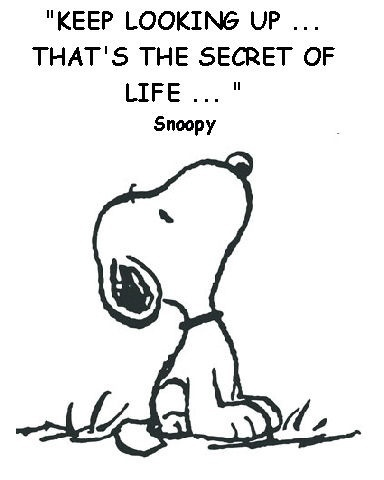
\includegraphics[scale=0.42]{back/snoopy2.jpg}
\end{flushright}
\end{figure*}
%\large{\em ``Every atom in your body came from a star that exploded. And, the atoms in your left hand probably came from a different star than your right hand. It really is the most poetic thing I know about physics: You are all stardust. You couldn't be here if stars hadn't exploded, because the elements - the carbon, nitrogen, oxygen, iron, all the things that matter for evolution and for life - weren't created at the beginning of time. They were created in the nuclear furnaces of stars, and the only way for them to get into your body is if those stars were kind enough to explode. [...] The stars died so that you could be here today."}


%\large {\em Dust if you must, but wouldn't it be better
%
%To paint a picture, or write a letter,
%
%Bake a cake, or plant a seed;
%
%Ponder the difference between want and need?
%
%\vspace{2ex}
%Dust if you must, but there's not much time,
%
%With rivers to swim, and mountains to climb;
%
%Music to hear, and books to read;
%
%Friends to cherish, and life to lead.
%
%\vspace{2ex}
%Dust if you must, but the world's out there
%
%With the sun in your eyes, and the wind in your hair;
%
%A flutter of snow, a shower of rain,
%
%This day will not come around again.
%
%\vspace{2ex}
%Dust if you must, but bear in mind,
%
%Old age will come and it's not kind.
%
%And when you go (and go you must)
%
%You, yourself, will make more dust.}

%\large {\em ``Cumulus clouds in the summer afternoon sky present a striking contrast of white against a bright blue sky.  During a sudden thundershower the primary and secondary rainbows display their multicolored arches.  Other colors in nature are the dark green of forest foliage and the red and orange hues of the Grand Canyon in early morning.  High in the mountains or on the desert when the air is clean one can clearly see dark patches in the bright band of the Milky Way.  Chimney smut turns all it touches to dirty blackness, and iridescent opal shimmers with a variety of colours''} 
%\\

\ \

\normalsize
%{- Lawrence M. Krauss}
%%{- Craig F. Bohren and Donald C. Huffman
%{- Rose Milligan}
%{\em Absorption and Scattering of Light by Small Particles}}
%\end{flushright}




\vspace*{\fill}

\vspace*{\fill}

\vspace*{\fill}

